\subsection{Layer Operating System}
The front-end, like the entire application, will be run on the browser and will therefore run on any operating system.

\subsection{Layer Software Dependencies}
The entire front-end will depend on Bootstrap, and the React library. The front-end will also depend on a consistent connection to the Query Manager on the Server layer.

\subsection{Login Subsystem}
The Login Subsystem will will provide an interface for user to login into the application. Users will be able to login with their email and password credentials or their Google accounts.

\begin{figure}[h!]
	\centering
 	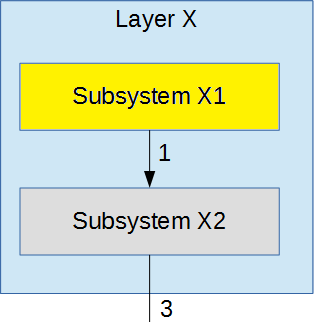
\includegraphics[width=0.60\textwidth]{images/subsystem}
 \caption{Example subsystem description diagram}
\end{figure}

\subsubsection{Subsystem Software Dependencies}
For a user to login with their Google accounts, the Login Subsystem will depend on the GoogleLogin library.

\subsubsection{Subsystem Programming Languages}
The Login Subsystem will be developed using, React.js, HTML, and CSS.

\subsubsection{Subsystem Data Processing}
If the user logs in using their email and password, they will enter their credentials in the respective places and click the login button. Upon the login buttoin being pressed, the Login Subsystem will send the user's credentials to the Query Manager in the backend layer. If the Login Subsystem receives a success signal, then the user will be redirected to the Home Page. If the Login Subsystem receives a failure signal, the Login Subsystem will display a failure message and prompt the user to re-enter their credentials.

If the user decides to login with their Google account, they will select the Google login button. The Login Subsystem will then call on the GoogleLogin API which users will login with. If the login is successful, the Login Subsystem will redirect the user to the Home Page. If the login fails, the user will be given an error message and prompted to re-enter their credentials.

%------------> Register 
\subsection{Register Subsystem}
The Register Subsystem will provide an interface for users to register for an account.

\begin{figure}[h!]
	\centering
 	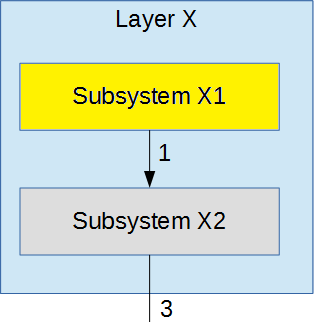
\includegraphics[width=0.60\textwidth]{images/subsystem}
 \caption{Example subsystem description diagram}
\end{figure}

\subsubsection{Subsystem Software Dependencies}
The Register Subsystem does not have any additional dependencies.

\subsubsection{Subsystem Programming Languages}
The Register Subsystem will be developed using, React.js, HTML, and CSS.

\subsubsection{Subsystem Data Processing}
After entering their password and unique email and username, the user will press the Register button. Upon the Register button being pressed, the Register Subsystem will capture the user entered information and send it to the Query Manager. If the Query Manager sends a success signal, the Register Subsystem will redirect the user to the Home Page. If the Query Manager sends a failure signal, the Register Subsystem will display an error message and prompt the user to re-enter their information.

%------------> Shopping List
\subsection{Shopping List Subsystem}

\begin{figure}[h!]
	\centering
 	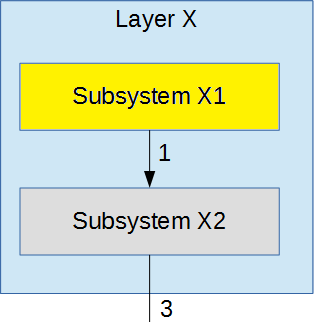
\includegraphics[width=0.60\textwidth]{images/subsystem}
 \caption{Example subsystem description diagram}
\end{figure}

\subsubsection{Subsystem Software Dependencies}
The Shopping List Subsystem has no additional dependencies.

\subsubsection{Subsystem Programming Languages}
The Shopping List Subsystem will be developed using, React.js, HTML, and CSS.

\subsubsection{Subsystem Data Processing}
The Shopping List Subsystem will retrieve the current user's shopping list from the Query Manager and display all relavent information.

%------------> Recipes
\subsection{Recipes Subsystem}

\begin{figure}[h!]
	\centering
 	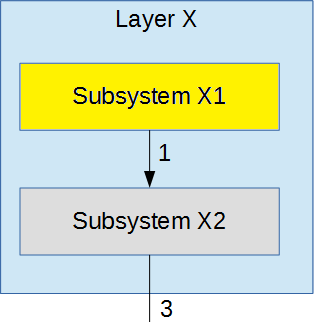
\includegraphics[width=0.60\textwidth]{images/subsystem}
 \caption{Example subsystem description diagram}
\end{figure}

\subsubsection{Subsystem Software Dependencies}
The Recipes Subsystem has no additional dependencies.

\subsubsection{Subsystem Programming Languages}
The Recipes Subsystem will be developed using, React.js, HTML, and CSS.

\subsubsection{Subsystem Data Processing}
The Recipes Subsystem will display all recipes retrieved by the Query Manager.

%------------> Meal Plan
\subsection{Meal Plan Subsystem}

\begin{figure}[h!]
	\centering
 	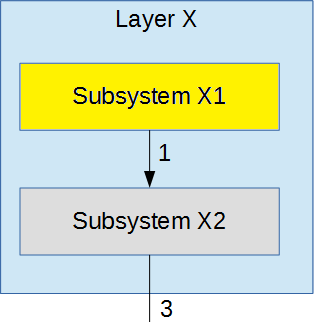
\includegraphics[width=0.60\textwidth]{images/subsystem}
 \caption{Example subsystem description diagram}
\end{figure}

\subsubsection{Subsystem Software Dependencies}
The Meal Plan Subsystem has no additional dependencies.

\subsubsection{Subsystem Programming Languages}
The Meal Plan Subsystem will be developed using, React.js, HTML, and CSS.

\subsubsection{Subsystem Data Processing}
The Meal Plan Subsystem will dislay of the current user's Meal Plans that are retrieved by the Query Manager.

%------------> Shop
\subsection{Shop Subsystem}

\begin{figure}[h!]
	\centering
 	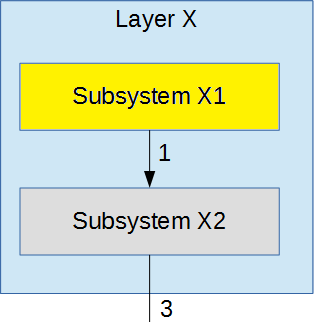
\includegraphics[width=0.60\textwidth]{images/subsystem}
 \caption{Example subsystem description diagram}
\end{figure}

\subsubsection{Subsystem Software Dependencies}
The Shop Subsystem depends on a consistent connection to the Shop Manager on the Server layer.

\subsubsection{Subsystem Programming Languages}
The Shop Subsystem will be developed using, React.js, HTML, and CSS.

\subsubsection{Subsystem Data Processing}
The Shop Subsystem will display all information that is calculated by the Shopping Manager.


